\subsection[Mechanizm działania (Jakub Wyka)]{Mechanizm działania}
Wymagania infrastruktury:
\begin{itemize}
    \item Raspberry Pi Zero z dostępem do internetu przez sieć wlan 
    \item Przewód USB – micro USB łączący Raspberry Pi Zero z testowanym komputerem    
\end{itemize}
Sposób działania:
Po odpowiedniej konfiguracji RPI0, testowany komputer automatycznie połączy się z nową siecią. Będzie ono widoczne jako połączenie Ethernet. W praktyce dostęp do internetu zapewniany będzie po kablu USB pomiędzy testowanym komputerem a RPI0, które będzie pełniło funkcję karty sieciowej.
\begin{figure}[H]
    \centering
    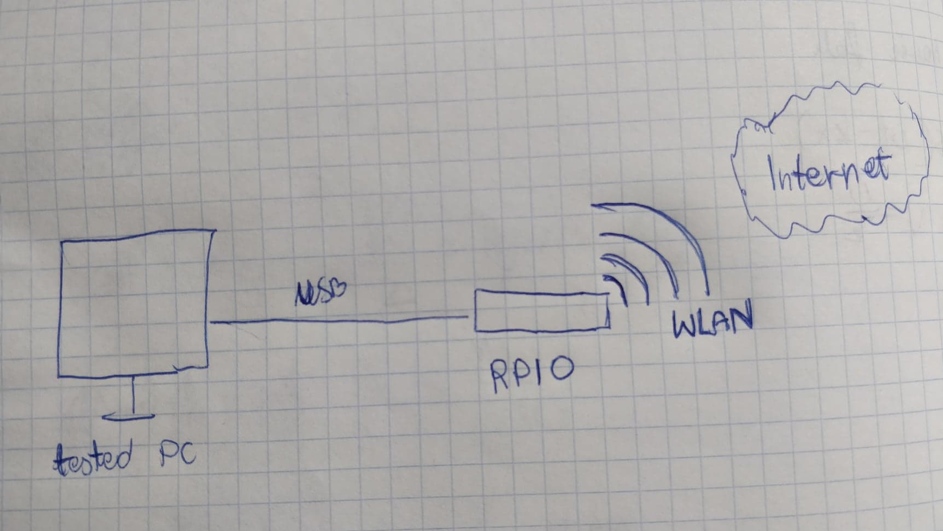
\includegraphics[width=\textwidth]{jw01}
    \caption{Schemat}
    \label{fig:ethmechanizm}
\end{figure}